\documentclass{article}

\usepackage[margin={2cm},a4paper]{geometry}

%% Move line apart a little (looks better)
\linespread{1.1}

%% Paragraphs have a bit of space in between and the first line is indented
\usepackage{parskip}
\setlength{\parindent}{0pt}

%% The left and right header
\usepackage{fancyhdr}
\pagestyle{fancy}
\rhead{\bfseries Tausch}
\lhead{}

\usepackage{tikz}

\usepackage{tipa}

\usepackage{hyperref}
\usepackage{float}

\usepackage{amsmath}

\usepackage{color, colortbl}

%% For source code
\usepackage{listings}
\lstset{language=C++,
    showstringspaces=false,
    basicstyle=\footnotesize,
    frame=single,
    texcl=true,
    numbers=left,
    numberstyle=\footnotesize,
    numbersep=5pt,
    numberblanklines=false,
    mathescape=false,
    breaklines=true,
    keywordstyle=\bfseries\color{green!40!black},
    commentstyle=\itshape\color{purple!40!black},
    identifierstyle=\color{blue},
    stringstyle=\color{orange},
    escapeinside={@}{@},
    tabsize=4}
\def\listingsfont{\ttfamily}
\def\lstlistingautorefname{Code}
\renewcommand{\lstlistingname}{Code}

\begin{document}

% \section*{Introduction}

\begin{center}\Huge\bfseries
    Tausch
\end{center}


Tausch (pronounced: [ta\textupsilon\textesh]) is a halo exchange library that provides a uniform interface for halo exchanges irrespective of the compute units involved in the data transfer.

\section{Glossary}

Some of the terms used in this document are as follows:
\begin{itemize}
    \item \textbf{local halo}: This is the data that is owned by the current MPI rank and needed by another (remote) MPI rank.
    \item \textbf{remote halo}: This is the data that is not owned by the current MPI rank but is needed from another MPI rank as halo data for its computations.
    \item \textbf{compute device} or \textbf{compute unit}: Referring to either the CPU or the GPU as both can do computations.
\end{itemize}

\section{What Tausch expects}

Tausch doesn't come with many expectations, it can work with a large variety of setups. One requirement is regarding the data layout in the arrays: The data is expected to be stored in one consecutive array, first along the $x$, second along the $y$, and third along the $z$ direction, as illustrated in \autoref{fig:datastorage}.

\begin{figure}[ht]\centering
    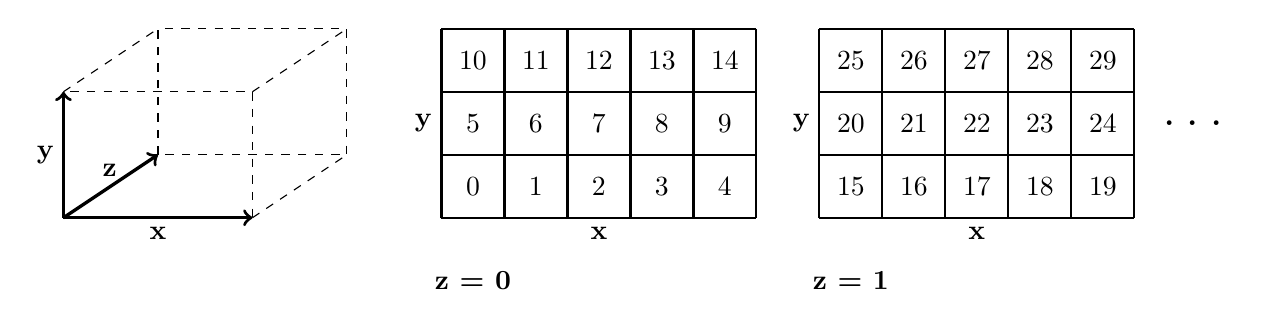
\begin{tikzpicture}[scale=0.8]

        \draw [dashed] (-6,0) rectangle (-3,2);
        \draw [dashed] (-4.5,1) rectangle (-1.5,3);
        \draw [dashed] (-6,2) -- (-4.5,3);
        \draw [dashed] (-3,2) -- (-1.5,3);
        \draw [dashed] (-3,0) -- (-1.5,1);

        \draw [very thick, ->] (-6,0) -- (-3,0);
        \draw [very thick, ->] (-6,0) -- (-6,2);
        \draw [very thick, ->] (-6,0) -- (-4.5,1);

        \node [below] at (-4.5,0) {\bfseries x};
        \node [left] at (-6,1) {\bfseries y};
        \node [above left] at (-5,0.5) {\bfseries z};

        % z = 0

        \draw [thick] (0,0) grid (5,3);

        \node at (0.5, 0.5) {0};
        \node at (1.5, 0.5) {1};
        \node at (2.5, 0.5) {2};
        \node at (3.5, 0.5) {3};
        \node at (4.5, 0.5) {4};

        \node at (0.5, 1.5) {5};
        \node at (1.5, 1.5) {6};
        \node at (2.5, 1.5) {7};
        \node at (3.5, 1.5) {8};
        \node at (4.5, 1.5) {9};

        \node at (0.5, 2.5) {10};
        \node at (1.5, 2.5) {11};
        \node at (2.5, 2.5) {12};
        \node at (3.5, 2.5) {13};
        \node at (4.5, 2.5) {14};

        \node [below] at (2.5, 0) {\bfseries x};
        \node [left] at (0, 1.5) {\bfseries y};

        \node at (0.5, -1) {\bfseries z = 0};


        % z = 1

        \draw [thick] (6,0) grid (11,3);

        \node at (6.5, 0.5) {15};
        \node at (7.5, 0.5) {16};
        \node at (8.5, 0.5) {17};
        \node at (9.5, 0.5) {18};
        \node at (10.5, 0.5) {19};

        \node at (6.5, 1.5) {20};
        \node at (7.5, 1.5) {21};
        \node at (8.5, 1.5) {22};
        \node at (9.5, 1.5) {23};
        \node at (10.5, 1.5) {24};

        \node at (6.5, 2.5) {25};
        \node at (7.5, 2.5) {26};
        \node at (8.5, 2.5) {27};
        \node at (9.5, 2.5) {28};
        \node at (10.5, 2.5) {29};

        \node [below] at (8.5, 0) {\bfseries x};
        \node [left] at (6, 1.5) {\bfseries y};

        \node at (6.5, -1) {\bfseries z = 1};

        \node at (12,1.5) {\huge \ldots};

    \end{tikzpicture}

    \caption{How Tausch expects the data to be stored \label{fig:datastorage}}

\end{figure}


This data array is also expected to contain the space required for remote halo data! Thus, the x, y, and z dimensions are expected to be larger (by the widths of the remote halo) than the dimensions of the actual subdomain owned by the rank. \autoref{fig:storewhat} illustrates this requirement.

\begin{figure}[ht]\centering
    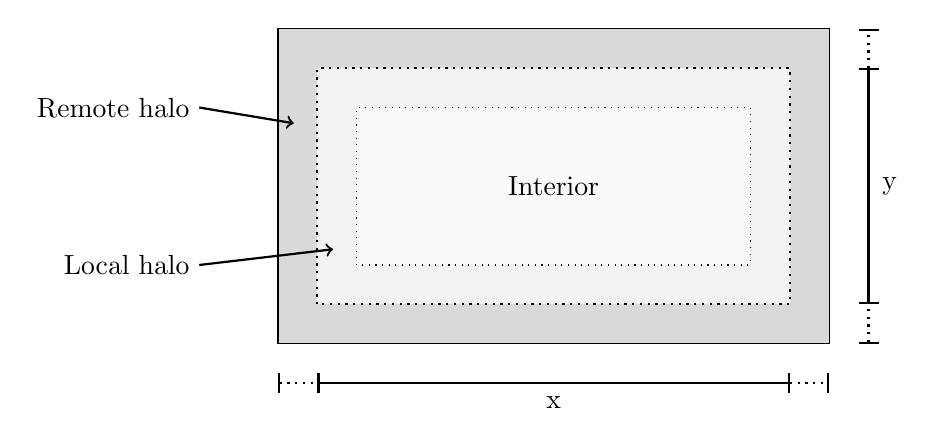
\begin{tikzpicture}
        \draw [fill=black!15] (0,0) rectangle (7,4);
        \draw [thick, dotted, fill=black!5] (0.5,0.5) rectangle (6.5,3.5);
        \draw [fill=black!2, dotted] (1,1) rectangle (6,3);

        \node [left] at (-1,3) {Remote halo};
        \draw [thick, ->] (-1,3) -- (0.2,2.8);
        \node [left] at (-1,1) {Local halo};
        \draw [thick, ->] (-1,1) -- (0.7,1.2);
        \node at (3.5,2) {Interior};

        \draw [thick, |-|] (0.5, -0.5) -- (6.5, -0.5);
        \node [below] at (3.5,-0.55) {x};
        \draw [thick, |-|] (7.5, 0.5) -- (7.5, 3.5);
        \node [right] at (7.55, 2) {y};

        \draw [thick, dotted, |-] (0,-0.5) -- (0.5,-0.5);
        \draw [thick, dotted, -|] (6.5,-0.5) -- (7,-0.5);

        \draw [thick, dotted, |-] (7.5, 0) -- (7.5, 0.5);
        \draw [thick, dotted, -|] (7.5, 3.5) -- (7.5, 4);
%         \node [right] at (8.2, 0.25) {halo width};
%         \node [right] at (8.2, 3.75) {halo width};

    \end{tikzpicture}
    \caption{What each rank needs to store \label{fig:storewhat}}
\end{figure}


Communication between a CPU and a GPU is currently only supported when both compute units live on the same MPI rank. There are two different ways this can be implemented on the user's end: 1) They can both live in the same thread and operate one after the other, or 2) They can live in seperate threads allowing them to run concurrently. A schematic way of how to realise computations on the CPU and GPU concurrently in seperate threads is shown in \autoref{fig:threadsschematic}:

\begin{figure}[ht]\centering
    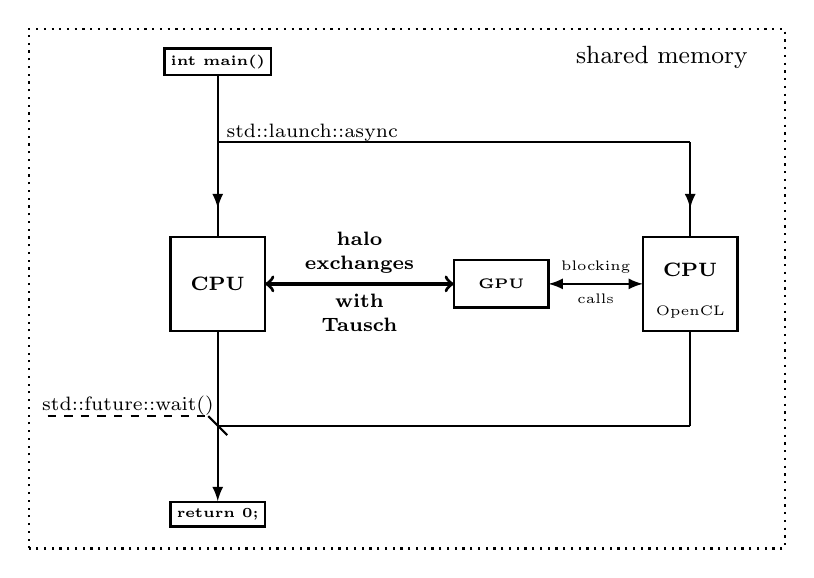
\begin{tikzpicture}[scale=1.2]

        % main thread
        \begin{scope}[thick, every node/.style={sloped,allow upside down}]

            \draw (0,4.7) -- (0,4);
            \node[above, draw=black, inner sep=0.8mm] at (0,4.7) {\tiny\bf int main()};
            \draw [-latex] (0,1) -- (0,0.2);
            \node[below, draw=black, inner sep=0.8mm] at (0,0.2) {\tiny\bf return 0;};

            \draw [dotted] (-2,-0.3) rectangle (6,5.2);
            \node at (4.7,4.9) {\small shared memory};

            % split
            \draw (0,4) -- (5, 4);
            \node [above] at (1,3.9) {\scriptsize std::launch::async};
            \draw [-latex] (5,4) -- (5,3.3);
            \draw (5,3.4) -- (5,3);
            \draw [-latex] (0,4) -- (0,3.3);
            \draw (0,3.4) -- (0,3);

            % CPU and GPU
            \draw (-0.5,3) rectangle (0.5,2);
            \draw (4.5,3) rectangle (5.5,2);
            \node at (0, 2.5) {\scriptsize\bfseries CPU};
            \node at (5, 2.65) {\scriptsize\bfseries CPU};
            \node at (5, 2.2) {\tiny OpenCL};

            % GPU
            \node [above] at (4,2.5) {\tiny blocking};
            \node [below] at (4,2.5) {\tiny calls};
            \draw [latex-latex] (3.5,2.5) -- (4.5,2.5);
            \draw (2.5,2.25) rectangle (3.5,2.75);
            \node at (3,2.5) {\tiny\bfseries GPU};

            % Tausch comm
            \draw [very thick, <->] (0.5, 2.5) -- (2.5, 2.5);
            \node [above] at (1.5, 2.8) {\scriptsize\bfseries halo};
            \node [above] at (1.5, 2.5) {\scriptsize\bfseries exchanges};
            \node [below] at (1.5, 2.5) {\scriptsize\bfseries with};
            \node [below] at (1.5, 2.25) {\scriptsize\bfseries Tausch};

            % rejoin
            \draw (5,2) -- (5,1);
            \draw (5,1) -- (0,1);
            \draw (0,1) -- (0,2);

            \draw [dashed] (-1.8,1.1) -- (-0.1,1.1);
            \draw (-0.1,1.1) -- (0.1,0.9);
            \node [above] at (-0.95,1) {\scriptsize std::future::wait()};

        \end{scope}

    \end{tikzpicture}
    \caption{Schematic of how to compute on CPU and GPU concurrently in seperate threads \label{fig:threadsschematic}}
\end{figure}

When the computations on the CPU and the GPU run in seperate threads, Tausch will make sure to properly synchronise the threads when communicating the halo data. If both are running in the same thread, then Tausch must be told to do any synchronisation, as this would otherwise lead to a deadlock.

\section{How Tausch works}\label{sec:howtauschworks}

If everything is set up matching Tausch's expectations, then the way Tausch performs a halo exchange is rather straight forward:

\begin{enumerate}
    \item First it extracts the local halo data that needs to be sent somewhere else into a dedicated send buffer. \autoref{fig:packintosend} shows an example of how it is done for a two-dimensional domain.
        \begin{figure}[ht]\centering
            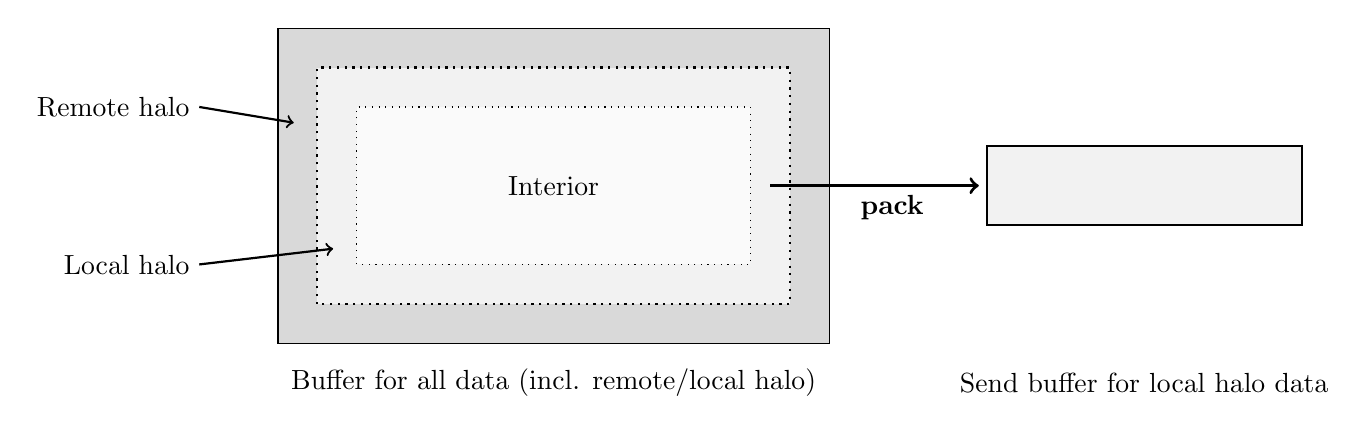
\begin{tikzpicture}
                \draw [fill=black!15] (0,0) rectangle (7,4);
                \draw [thick, dotted, fill=black!5] (0.5,0.5) rectangle (6.5,3.5);
                \draw [fill=black!2, dotted] (1,1) rectangle (6,3);

                \node [left] at (-1,3) {Remote halo};
                \draw [thick, ->] (-1,3) -- (0.2,2.8);
                \node [left] at (-1,1) {Local halo};
                \draw [thick, ->] (-1,1) -- (0.7,1.2);
                \node at (3.5,2) {Interior};

                \draw [thick, fill=black!5] (9,1.5) rectangle (13,2.5);

                \draw [very thick, ->] (6.25,2) -- (8.9,2);
                \node [below] at (7.8,2) {\bfseries pack};

                \node at (3.5,-0.5) {Buffer for all data (incl. remote/local halo)};
                \node at (11,-0.5) {Send buffer for local halo data};
            \end{tikzpicture}
            \caption{Packing local halo data into dedicated send buffer \label{fig:packintosend}}
        \end{figure}

        Tausch does not know by itself where to look for the local halo data. It relies on the user telling it the data locations. This enables Tausch to allow for maximum flexibility.

    \item The packed data is then sent to the receiver. How exactly this is done depends on the type of compute devices the data lives on (both sending and receiving end):
        \begin{enumerate}
            \item \textbf{CPU to CPU}: When data is sent from one CPU to another, then this is achieved using simple MPI routines. The very first time data is sent between two CPUs, Tausch uses \emph{MPI\_Send\_init} and \emph{MPI\_Recv\_init} to establish persistent communication channels between the two compute units. Every subsequent time data needs to be communicated between these two compute units, the same channels are used.
            \item \textbf{CPU to GPU}: In this case both compute units operate on the very same subdomain, with the GPU handling some subset of that subdomain. This allows the two threads handling the computations on the CPU and on the GPU to access memory shared between them. Thus, to send data from the CPU to the GPU, Tausch takes advantage of this and simply writes the halo data to be communicated to a shared buffer (using atomic operations). The receiving thread reads the data from the very same buffer (using atomic operations) and uploads the data to the GPU using OpenCL.
            \item \textbf{GPU to CPU}: To get the data off the GPU requires first the download of the data from the GPU using OpenCL. Again taking advantage of shared memory, Tausch then writes the data to a shared buffer (using atomic operations), which then is read by the receiving thread (using atomic operations).
            \item \textbf{GPU to GPU}: Sending data from one GPU to another (both living on different MPI ranks) requires a combinations of the above types of communication. First the required data is downloaded from the sending GPU using OpenCL, sent to the receiving MPI rank using standard MPI functions, and then uploaded to the receiving GPU using OpenCL.
        \end{enumerate}
    \item The final step to complete the communication step is the unpacking of the data. The received data is stored in a dedicated receive buffer and needs to be copied into the right locations (the remote halo area) inside the main data buffer, as illustrated by \autoref{fig:packfromrecv} for a two-dimensional example.
        \begin{figure}[ht]\centering
            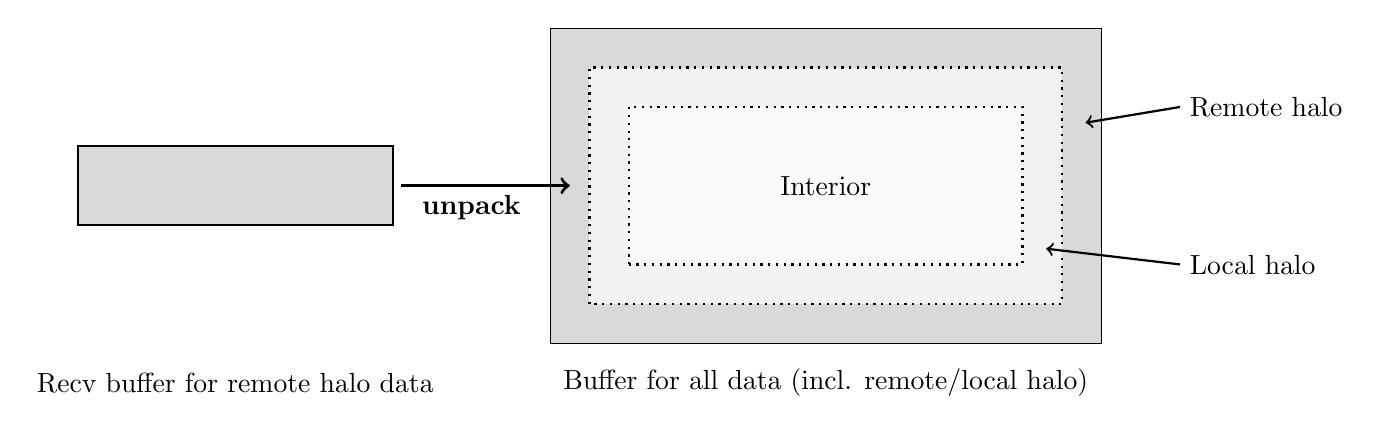
\begin{tikzpicture}
                \draw [fill=black!15] (7,0) rectangle (14,4);
                \draw [thick, dotted, fill=black!5] (7.5,0.5) rectangle (13.5,3.5);
                \draw [thick, dotted, fill=black!2] (8,1) rectangle (13,3);

                \node [right] at (15,3) {Remote halo};
                \draw [thick, ->] (15,3) -- (13.8,2.8);
                \node [right] at (15,1) {Local halo};
                \draw [thick, ->] (15,1) -- (13.3,1.2);
                \node at (10.5,2) {Interior};
%
                \draw [thick, fill=black!15] (1,1.5) rectangle (5,2.5);
%
                \draw [very thick, ->] (5.1,2) -- (7.25,2);
                \node [below] at (6,2) {\bfseries unpack};
%
                \node at (10.5,-0.5) {Buffer for all data (incl. remote/local halo)};
                \node at (3,-0.5) {Recv buffer for remote halo data};
            \end{tikzpicture}
            \caption{Unpacking of remote halo data out of dedicated recv buffer \label{fig:packfromrecv}}
        \end{figure}

        Tausch does not know by itself where to write the remote halo data to. It relies on the user telling it the data locations. This enables Tausch to allow for maximum flexibility.

\end{enumerate}



\section{API overview}

The API of Tausch very closely resembles the steps of how Tausch works (see \autoref{sec:howtauschworks}), though it needs to be broken down into a few additional steps.

\begin{enumerate}
    \item During setup, Tausch needs to be told which halo regions exist and where they are in the respective buffers. For this purpose Tausch provides a struct called \emph{TauschHaloSpec}. This struct contains information about:
    \begin{table}[ht]\centering
    \begin{tabular}{|l|l|}
        \hline
        \rowcolor{black!10}
        & \bfseries struct members\\
        \hline
        the underying buffer & bufferWidth, bufferHeight, bufferDepth\\
        the starting location of the halo & haloX, haloY, haloZ\\
        the size of the halo region & haloWidth, haloHeight, haloDepth\\
        the receiving/sending MPI rank & remoteMpiRank\\
        \hline
    \end{tabular}
    \end{table}

    The field \emph{remoteMpiRank} is used for both the receiving and sending MPI rank, as Tausch needs to be told both about the local halo (in which case \emph{remoteMpiRank} contains the receiving MPI rank) and the remote halo (in which case \emph{remoteMpiRank} contains the sending MPI rank). This struct can be constructed in two ways:
    \begin{enumerate}
        \item Like any other struct in C/C++, it can simply be instantiated and filled by setting values to its members:
        \begin{lstlisting}
TauschHaloSpec halospec;
halospec.bufferWidth = 100; halospec.bufferHeight = 100;
halospec.haloX = 0;         halospec.haloY = 0;
halospec.haloWidth = 100;   halospec.haloHeight = 2;
halospec.remoteMpiRank = 1;
        \end{lstlisting}
        \item Tausch provides the possibility to create such an object and fill it with the right data all with one function call:
        \begin{lstlisting}
TauschHaloSpec halospec = tausch.createFilledHaloSpec2D(100, 100, 0, 0, 100, 2, 1);
        \end{lstlisting}
    \end{enumerate}

    Once the structs are constructed, they are set using either the \emph{setLocalHaloInfo} or \emph{setRemoteHaloInfo} function. Both require as first parameter the number of halo regions (i.e., the number of structs) and as second function parameter they require an array containing exactly that many \emph{TauschHaloSpec} structs.

    \textbf{The order in which Tausch is told about the halo regions is important!} The position of a halo region in this order is its id (i.e., the first halo region has an id of 0, the second one an id of 1, etc.).

    \item Once the configuration of all the halo regions has been set and some halo data needs to be communicated, then the data needed for the remote halo of another MPI rank first has to be packed into a dedicated send buffer. In Tausch, this is done with a call to \emph{packSendBuffer}. It needs to be told
    \begin{enumerate}
        \item Which halo region it is supposed to pack (the halo id)
        \item Which buffer it is supposed to pack (the buffer id)
        \item A pointer to the actual buffer
        \item And the subregion of the total halo region that is to be packed. This is a simple struct called \emph{TauschPackRegion} that contains the following information:
        \begin{table}[ht]\centering
        \begin{tabular}{|l|l|}
            \hline
            \rowcolor{black!10}
            & \bfseries struct members\\
            \hline
            the starting location of the pack region & x, y, z \\
            the dimensions of the pack region & width, height, depth \\
            \hline
        \end{tabular}
        \end{table}

        Similarly as with the struct \emph{TauschHaloSpec}, this struct can be created either like any C/C++ struct or with the Tausch member function \emph{createFilledPackRegion}:
        \begin{lstlisting}
TauschPackRegion halospec = tausch.createFilledPackRegion(0, 0, 100, 2);
        \end{lstlisting}

        \textbf{This last parameter (the struct) is optional.} If it is not passed on, then Tausch will simply pack the full halo region into the send buffer.
    \end{enumerate}


    \item In order for the halo data to be received by the remoteMpiRank, the remote MPI rank has to be listening (i.e., its receives need to be posted). This is done by calling \emph{postReceive}. It needs to be told
    \begin{enumerate}
        \item For which halo region to listen (the halo id)
        \item What message tag to use. The message tag can be though of like an MPI tag in MPI communications (in fact, for CPU/CPU communication is is used as the MPI tag).
    \end{enumerate}
    If the receives of all the halo regions are to be posted, this can also be done using the \emph{postAllReceives} function. It expects a single parameter only, an array of message tags. The first message tag is used for the halo with id 0, the second tag for the halo with id 1, etc.

    For both functions, the message tag only needs to be set the first time the receives are posted. For each consecutive time Tausch can re-use the already set tags. This can be achieved by either not passing any message tag, or passing a message tag with value -1 (resp., an array filled with all -1).

    The exact point in the code when the receives are posted is not important, as long as they are posted \textbf{before} the data is sent off.

    \item Once the data that needs to be communicated has been packed it can be sent off. This is done by calling the \emph{send} function. It needs to be told
    \begin{enumerate}
        \item Which halo region to send off (the halo id)
        \item What message tag to use. This message tag must correspond to the message tag with which the receiving MPI rank is listening!
    \end{enumerate}

    \item Receiving the data for some remote halo is done by calling the \emph{recv} function. This function does nothing except ensuring that the wanted data has arrived in the dedicated receive buffers. It only needs to be told for which halo id to ensure this.

    \item The final step in communicating halo data is unpacking the received data from the dedicated receive buffer into the actual data buffer. This is done using the function \emph{unpackRecvBuffer}. It requires the same types of information as the \emph{packSendBuffer}:
    \begin{enumerate}
        \item Which halo region the unpacked data corresponds to (the halo id)
        \item Which buffer will receive the data (the buffer id)
        \item A pointer to the actual buffer
        \item And the subregion of the total halo region that is to be unpacked. This is a simple struct called \emph{TauschPackRegion} that contains the following information:
        \begin{table}[ht]\centering
        \begin{tabular}{|l|l|}
            \hline
            \rowcolor{black!10}
            & \bfseries struct members\\
            \hline
            the starting location of the pack region & x, y, z \\
            the dimensions of the pack region & width, height, depth \\
            \hline
        \end{tabular}
        \end{table}

        Similarly as with the struct \emph{TauschHaloSpec}, this struct can be created either like any C/C++ struct or with the Tausch member function \emph{createFilledPackRegion}:
        \begin{lstlisting}
TauschPackRegion halospec = tausch.createFilledPackRegion(0, 0, 100, 2);
        \end{lstlisting}

        \textbf{This last parameter (the struct) is optional.} If it is not passed on, then Tausch will simply unpack the full halo region from the receive buffer into the data buffer.
    \end{enumerate}
\end{enumerate}

Steps 2 to 6 need to be repeated for each full communication step. The first step is only necessary once during the set up phase.

The API distinguishes between the 1D, 2D and the 3D version by a suffix to the respective function names. It does the same with distinguishing the communication paths. In the case of the \emph{packSendBuffer} function, all the available function variants are:

\begin{table}[ht]\centering
    \begin{tabular}{|>{\columncolor{black!10}}c|c|c|c|}
        \hline
        \rowcolor{black!10}
        & \bfseries 1D & \bfseries 2D & \bfseries 3D\\
        \hline
        \bfseries CPU $\rightarrow$ CPU & packSendBuffer1D\_CwC & packSendBuffer2D\_CwC & packSendBuffer3D\_CwC\\
        \bfseries CPU $\rightarrow$ GPU & packSendBuffer1D\_CwG & packSendBuffer2D\_CwG & packSendBuffer3D\_CwG\\
        \bfseries GPU $\rightarrow$ CPU & packSendBuffer1D\_GwC & packSendBuffer2D\_GwC & packSendBuffer3D\_GwC\\
        \bfseries GPU $\rightarrow$ GPU & packSendBuffer1D\_GwG & packSendBuffer2D\_GwG & packSendBuffer3D\_GwG\\
        \hline
    \end{tabular}
\end{table}

\end{document}
